%%%%%%%%%%%%%%%%%%%%%%%%%%%%%%%%%%%%%%%%%
% Lachaise Assignment
% LaTeX Template
% Version 1.0 (26/6/2018)
%
% This template originates from:
% http://www.LaTeXTemplates.com
%
% Authors:
% Marion Lachaise & François Févotte
% Vel (vel@LaTeXTemplates.com)
%
% License:
% CC BY-NC-SA 3.0 (http://creativecommons.org/licenses/by-nc-sa/3.0/)
% 
%%%%%%%%%%%%%%%%%%%%%%%%%%%%%%%%%%%%%%%%%

%----------------------------------------------------------------------------------------
%	PACKAGES AND OTHER DOCUMENT CONFIGURATIONS
%----------------------------------------------------------------------------------------

\documentclass{article}


%
\usepackage{indentfirst}
\usepackage{amsmath}
\usepackage{graphicx}
\usepackage{float}

% 


%%%%%%%%%%%%%%%%%%%%%%%%%%%%%%%%%%%%%%%%%
% Lachaise Assignment
% Structure Specification File
% Version 1.0 (26/6/2018)
%
% This template originates from:
% http://www.LaTeXTemplates.com
%
% Authors:
% Marion Lachaise & François Févotte
% Vel (vel@LaTeXTemplates.com)
%
% License:
% CC BY-NC-SA 3.0 (http://creativecommons.org/licenses/by-nc-sa/3.0/)
% 
%%%%%%%%%%%%%%%%%%%%%%%%%%%%%%%%%%%%%%%%%

%----------------------------------------------------------------------------------------
%	PACKAGES AND OTHER DOCUMENT CONFIGURATIONS
%----------------------------------------------------------------------------------------

\usepackage{amsmath,amsfonts,stmaryrd,amssymb} % Math packages

\usepackage{enumerate} % Custom item numbers for enumerations

\usepackage[ruled]{algorithm2e} % Algorithms

\usepackage[framemethod=tikz]{mdframed} % Allows defining custom boxed/framed environments

\usepackage{listings} % File listings, with syntax highlighting
\lstset{
	basicstyle=\ttfamily, % Typeset listings in monospace font
}

%----------------------------------------------------------------------------------------
%	DOCUMENT MARGINS
%----------------------------------------------------------------------------------------

\usepackage{geometry} % Required for adjusting page dimensions and margins

\geometry{
	paper=a4paper, % Paper size, change to letterpaper for US letter size
	top=2.5cm, % Top margin
	bottom=3cm, % Bottom margin
	left=2.5cm, % Left margin
	right=2.5cm, % Right margin
	headheight=14pt, % Header height
	footskip=1.5cm, % Space from the bottom margin to the baseline of the footer
	headsep=1.2cm, % Space from the top margin to the baseline of the header
	%showframe, % Uncomment to show how the type block is set on the page
}

%----------------------------------------------------------------------------------------
%	FONTS
%----------------------------------------------------------------------------------------

\usepackage[utf8]{inputenc} % Required for inputting international characters
\usepackage[T1]{fontenc} % Output font encoding for international characters

\usepackage{XCharter} % Use the XCharter fonts

%----------------------------------------------------------------------------------------
%	COMMAND LINE ENVIRONMENT
%----------------------------------------------------------------------------------------

% Usage:
% \begin{commandline}
%	\begin{verbatim}
%		$ ls
%		
%		Applications	Desktop	...
%	\end{verbatim}
% \end{commandline}

\mdfdefinestyle{commandline}{
	leftmargin=10pt,
	rightmargin=10pt,
	innerleftmargin=15pt,
	middlelinecolor=black!50!white,
	middlelinewidth=2pt,
	frametitlerule=false,
	backgroundcolor=black!5!white,
	frametitle={Command Line},
	frametitlefont={\normalfont\sffamily\color{white}\hspace{-1em}},
	frametitlebackgroundcolor=black!50!white,
	nobreak,
}

% Define a custom environment for command-line snapshots
\newenvironment{commandline}{
	\medskip
	\begin{mdframed}[style=commandline]
}{
	\end{mdframed}
	\medskip
}

%----------------------------------------------------------------------------------------
%	FILE CONTENTS ENVIRONMENT
%----------------------------------------------------------------------------------------

% Usage:
% \begin{file}[optional filename, defaults to "File"]
%	File contents, for example, with a listings environment
% \end{file}

\mdfdefinestyle{file}{
	innertopmargin=1.6\baselineskip,
	innerbottommargin=0.8\baselineskip,
	topline=false, bottomline=false,
	leftline=false, rightline=false,
	leftmargin=2cm,
	rightmargin=2cm,
	singleextra={%
		\draw[fill=black!10!white](P)++(0,-1.2em)rectangle(P-|O);
		\node[anchor=north west]
		at(P-|O){\ttfamily\mdfilename};
		%
		\def\l{3em}
		\draw(O-|P)++(-\l,0)--++(\l,\l)--(P)--(P-|O)--(O)--cycle;
		\draw(O-|P)++(-\l,0)--++(0,\l)--++(\l,0);
	},
	nobreak,
}

% Define a custom environment for file contents
\newenvironment{file}[1][File]{ % Set the default filename to "File"
	\medskip
	\newcommand{\mdfilename}{#1}
	\begin{mdframed}[style=file]
}{
	\end{mdframed}
	\medskip
}

%----------------------------------------------------------------------------------------
%	NUMBERED QUESTIONS ENVIRONMENT
%----------------------------------------------------------------------------------------

% Usage:
% \begin{question}[optional title]
%	Question contents
% \end{question}

\mdfdefinestyle{question}{
	innertopmargin=1.2\baselineskip,
	innerbottommargin=0.8\baselineskip,
	roundcorner=5pt,
	nobreak,
	singleextra={%
		\draw(P-|O)node[xshift=1em,anchor=west,fill=white,draw,rounded corners=5pt]{%
		Question \theQuestion\questionTitle};
	},
}

\newcounter{Question} % Stores the current question number that gets iterated with each new question

% Define a custom environment for numbered questions
\newenvironment{question}[1][\unskip]{
	\bigskip
	\stepcounter{Question}
	\newcommand{\questionTitle}{~#1}
	\begin{mdframed}[style=question]
}{
	\end{mdframed}
	\medskip
}

%----------------------------------------------------------------------------------------
%	WARNING TEXT ENVIRONMENT
%----------------------------------------------------------------------------------------

% Usage:
% \begin{warn}[optional title, defaults to "Warning:"]
%	Contents
% \end{warn}

\mdfdefinestyle{warning}{
	topline=false, bottomline=false,
	leftline=false, rightline=false,
	nobreak,
	singleextra={%
		\draw(P-|O)++(-0.5em,0)node(tmp1){};
		\draw(P-|O)++(0.5em,0)node(tmp2){};
		\fill[black,rotate around={45:(P-|O)}](tmp1)rectangle(tmp2);
		\node at(P-|O){\color{white}\scriptsize\bf !};
		\draw[very thick](P-|O)++(0,-1em)--(O);%--(O-|P);
	}
}

% Define a custom environment for warning text
\newenvironment{warn}[1][Warning:]{ % Set the default warning to "Warning:"
	\medskip
	\begin{mdframed}[style=warning]
		\noindent{\textbf{#1}}
}{
	\end{mdframed}
}

%----------------------------------------------------------------------------------------
%	INFORMATION ENVIRONMENT
%----------------------------------------------------------------------------------------

% Usage:
% \begin{info}[optional title, defaults to "Info:"]
% 	contents
% 	\end{info}

\mdfdefinestyle{info}{%
	topline=false, bottomline=false,
	leftline=false, rightline=false,
	nobreak,
	singleextra={%
		\fill[black](P-|O)circle[radius=0.4em];
		\node at(P-|O){\color{white}\scriptsize\bf i};
		\draw[very thick](P-|O)++(0,-0.8em)--(O);%--(O-|P);
	}
}

% Define a custom environment for information
\newenvironment{info}[1][Info:]{ % Set the default title to "Info:"
	\medskip
	\begin{mdframed}[style=info]
		\noindent{\textbf{#1}}
}{
	\end{mdframed}
}
 % Include the file specifying the document structure and custom commands

%----------------------------------------------------------------------------------------
%	ASSIGNMENT INFORMATION
%----------------------------------------------------------------------------------------

\title{CS223A - Introduction to Robotics - Homework \#2} % Title of the assignment

\author{Yunsen Xing \\
\texttt{Autonomous Systems and Intelligent Robots} \\
\texttt{yunsen@kth.se}} % Author name and email address
\date{KTH Royal Institute of Technology \&\& Aalto University --- \today}
% \date{KTH Royal Institute of Technology --- 23$^{rd}$ August 2025}
% University, school and/or department name(s) and a date

%----------------------------------------------------------------------------------------

\begin{document}

\maketitle % Print the title

%----------------------------------------------------------------------------------------
%	Question 1
%----------------------------------------------------------------------------------------

\section*{Question 1}
\begin{enumerate}
    \begin{align*}
        T_{2}' &= T_{1}T_{2}T_{1}^{-1} \\
        T_{3}' &= T_{1}T_{2}T_{3}(T_{1}T_{2})^{-1} \\
        T_{4}' &= T_{1}T_{2}T_{3}T_{4}(T_{1}T_{2}T_{3})^{-1}
    \end{align*}
    \texttt{Total displacement = }
    \begin{align*}
        T_{4}'T_{3}'T_{2}'T_{1} &= T_{1}T_{2}T_{3}T_{4}(T_{1}T_{2}T_{3})^{-1}T_{1}T_{2}T_{3}(T_{1}T_2)^{-1}T_{1}T_{2}T_{1}^{-1}T_{1} \\
        &=
        T_{1}T_{2}T_{3}T_{4}
    \end{align*}
\end{enumerate}

\section*{Question 2}
\begin{figure}
    \centering
    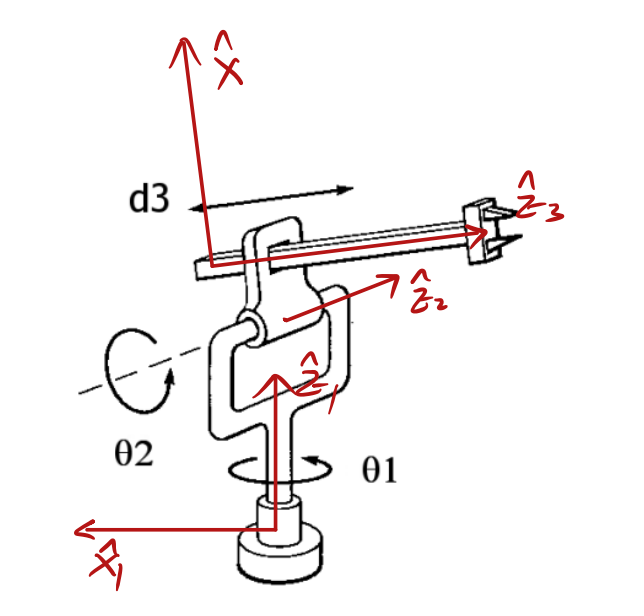
\includegraphics[width=0.4\linewidth]{picture/Question2.png}
    \caption{Question 2}
    \label{fig:placeholder}
\end{figure}

\texttt{DH parameters:}
\begin{enumerate}
    \[
        \begin{bmatrix}
            \cos{\theta_{i}} & -\sin{\theta_{i}} & 0 & a_{i-1} \\
            \sin{\theta_{i}}\cos{\alpha_{i-1}} & \cos{\theta_{i}}\cos{\alpha_{i-1}} & -\sin{\alpha_{i-1}} & -\sin{\alpha_{i-1}}d_{i} \\
            \sin{\theta_{i}\sin{\alpha_{i-1}}} & \cos{\theta_{i}\sin{\alpha_{i-1}}} & \cos{\alpha_{i-1}} & \cos{\alpha_{i-1}}d_{i} \\
            0 & 0 & 0 & 1
        \end{bmatrix}
    \]
\end{enumerate}

\begin{table}[t]
\centering
\begin{tabular}{|c|c|c|c|c|}
\hline
$i$ & $\alpha_{i-1}$ & $a_{i-1}$ & $d_{i}$ & $\theta_{i}$ \\ \hline
1  & 0  & 0  & 0  & $\theta_{1}$  \\ \hline
2  & $90^\circ$  & 0  & 0  & $\theta_{2}$  \\ \hline
3  & $90^\circ$  & $a_{2}$  & $d_{3}$  & 0  \\ \hline
\end{tabular}
\caption{the answer to question 2}
\label{tab:mytable}
\end{table}

\begin{enumerate}
    \[
        {}^{0}_{1}T = 
        \begin{bmatrix}
            \cos{\theta_{1}} & -\sin{\theta_{1}} & 0 & 0 \\
            \sin{\theta_{1}} & \cos{\theta_{1}} & 0 & 0 \\
            0 & 0 & 1 & 0 \\
            0 & 0 & 0 & 1
        \end{bmatrix}
    \]
    \[
        {}^{1}_{2}T = 
        \begin{bmatrix}
            \cos{\theta_{2}} & -\sin_{\theta_{2}} & 0 & 0 \\
            0 & 0 & -1 & 0 \\
            \sin{\theta_{2}} & \cos{\theta_{2}} & 0 & 0 \\
            0 & 0 & 0 & 1
        \end{bmatrix}
    \]
    \[
        {}^{2}_{3}T = 
        \begin{bmatrix}
            1 & 0 & 0 & a_{2} \\
            0 & 0 & -1 & -d_{3} \\
            0 & 1 & 0 & 0 \\
            0 & 0 & 0 & 1
        \end{bmatrix}
    \]

        \begin{align*}
            \therefore{}^{3}_{0}T &= {}^{1}_{0}T{}^{1}_{2}T{}^{2}_{3}T \\
            &=
            \begin{bmatrix}
                \cos{\theta_{1}} & -\sin{\theta_{1}} & 0 & 0 \\
                \sin{\theta_{1}} & \cos{\theta_{1}} & 0 & 0 \\
                0 & 0 & 1 & 0 \\
                0 & 0 & 0 & 1
            \end{bmatrix}
            \begin{bmatrix}
                \cos{\theta_{2}} & -\sin{\theta_{2}} & 0 & 0 \\
                0 & 0 & -1 & 0 \\
                \sin{\theta_{2}} & \cos{\theta_{2}} & 0 & 0 \\
                0 & 0 & 0 & 1
            \end{bmatrix}
            \begin{bmatrix}
                1 & 0 & 0 & a_{2} \\
                0 & 0 & -1 & -d_{3} \\
                0 & 1 & 0 & 0 \\
                0 & 0 & 0 & 1
            \end{bmatrix}
            \\
            &=
            \begin{bmatrix}
                \cos{\theta_{1}}\cos{\theta_{2}} & -\cos{\theta_{1}}\sin{\theta_{2}} & \sin{\theta_{1}} & 0 \\
                \sin{\theta_{1}}\cos{\theta_{2}} & -\sin{\theta_{1}}\sin{\theta_{2}} & -\cos{\theta_{1}} & 0 \\
                \sin{\theta_{2}} & \cos{\theta_{2}} & 0 & 0 \\
                0 & 0 & 0 & 1
            \end{bmatrix}
            \begin{bmatrix}
                1 & 0 & 0 & a_{2} \\
                0 & 0 & -1 & -d_{3} \\
                0 & 1 & 0 & 0 \\
                0 & 0 & 0 & 1
            \end{bmatrix}
            \\
            &= 
            \begin{bmatrix}
                \cos{\theta_{1}}\cos{\theta_{2}} & \sin{\theta_{1}} & \cos{\theta_{1}}\sin{\theta_{2}} & a_{2}\cos{\theta_{1}}\cos{\theta_{2}} + d_{3}\cos{\theta_{1}}\sin{\theta_{2}} \\
                \sin{\theta_{1}}\cos{\theta_{2}} & -\cos{\theta_{1}} & \sin{\theta_{1}}\sin{\theta_{2}} &  a_{2}\sin{\theta_{1}}\cos{\theta_{2}} + d_{3}\sin{\theta_{1}}\sin{\theta_2} \\
                \sin{\theta_{2}} & 0 & -\cos{\theta_{2}} & a_{2}\sin{\theta_[2]} - d_{3}\cos{\cos{\theta_{2}}} \\
                0 & 0 & 0 & 1
            \end{bmatrix}
        \end{align*}
\end{enumerate}

\section*{Another Example}
\begin{figure}[H]
    \centering
    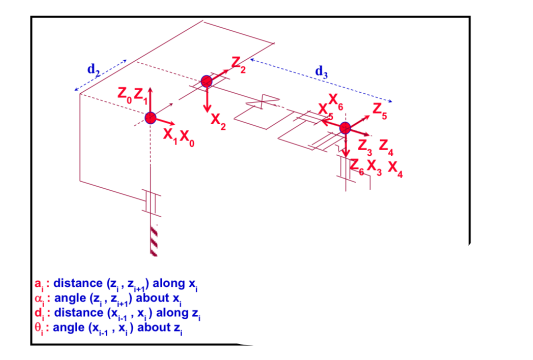
\includegraphics[width=0.5\linewidth]{picture/Example.png}
    \caption{Question 3}
    \label{fig:placeholder}
\end{figure}

\begin{table}[H]
\centering
\begin{tabular}{|c|c|c|c|c|}
\hline
$i$ & $\alpha_{i-1}$ & $a_{i-1}$ & $d_{i}$ & $\theta_{i}$ \\ \hline
1  & 0  & 0  & 0  & $\theta_{1}$  \\ \hline
2  & $-90^\circ$  & 0  & $d_{2}$  & $\theta_{2}$  \\ \hline
3  & $90^\circ$  & 0  & $d_{3}$  & 0  \\ \hline
4  & 0 & 0 & 0  & 0  \\ \hline
5  & $-90^\circ$  & 0  & 0 & $\theta_{5}$  \\ \hline
6  & $90^\circ$  & 0  & 0  & $\theta_{6}$ \\ \hline
\end{tabular}
\caption{the answer to the example}
\label{tab:mytable}
\end{table}

\section*{Question 3}
\begin{figure}[H]
    \centering
    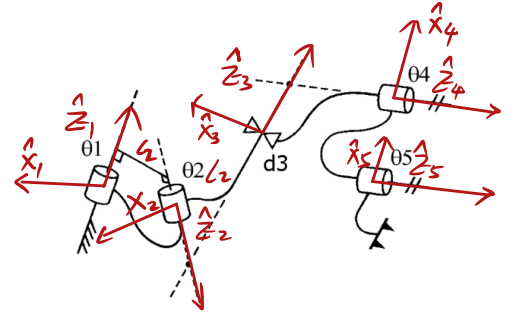
\includegraphics[width=0.5\linewidth]{picture/Question3.png}
    \caption{Question 3}
    \label{fig:placeholder}
\end{figure}

\begin{table}[H]
    \centering
    \begin{tabular}{|c|c|c|c|c|}
    \hline
         $i$ & $\alpha_{i-1}$ & $a_{i-1}$ & $d_{i}$ & $\theta_{i}$ \\ \hline
         1 & 0 & 0 & 0 & $\theta_{1}$ \\ \hline
         2 & $\alpha_{1}$ & $a_{1}$ & $d_{2}$ & $\theta_{2}$ \\ \hline
         3 & $\alpha_{2}$ & 0 & $d_{3}$ & $\theta_{3}$ \\ \hline
         4 & $\alpha_{3}$ & 0 & $d_{4}$ & $\theta_{4}$ \\ \hline
         5 & 0 & $a_{4}$ & 0 & $\theta_{5}$ \\ \hline
    \end{tabular}
    \caption{the answer to question 3}
    \label{tab:placeholder}
\end{table}


\end{document}
